\chapter{Radiation Damage to the ATLAS Pixel Detector}
\label{chap:digi}

The goal of this Chapter is to present a model for radiation damage to silicon sensors that is fast enough to be incorporated directly into the simulation of \textit{digitization}: the conversion from energy depositions from charged particles to digital signals sent from module front ends to the detector readout system.  Figure~\ref{fig:atlassim} shows the flowchart of the ATLAS Monte Carlo simulation, from 
event generation to analysis; digitization step intervenes before reconstruction.


\begin{figure}[!htpb]
\centering
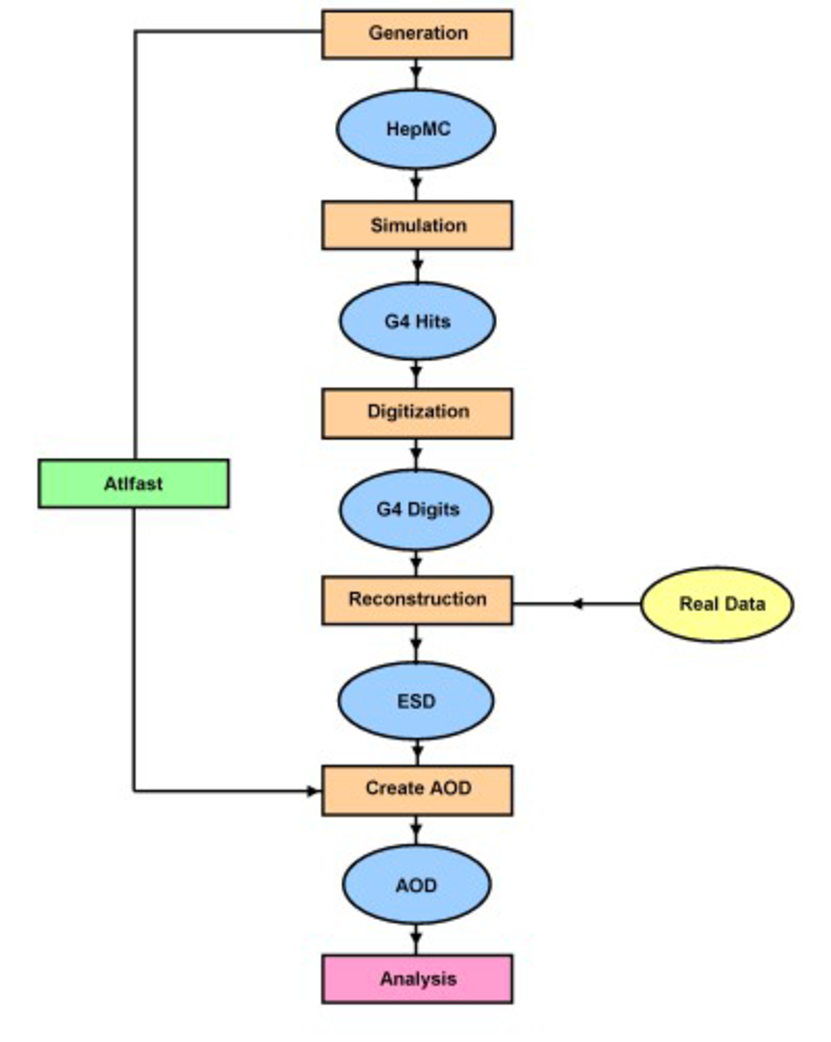
\includegraphics[height=0.45\textheight]{atlassim.pdf}
\caption{\label{fig:atlassim}Flowchart of Monte Carlo simulation in ATLAS.}
\end{figure}

 
After introducing the motivations and the the fluences predictions for the actual detector in 
Section~\ref{sec:expflu}, a model of charge deposition and measurement that includes radiation 
damage effects is documented in Section~\ref{sec:fullmodel}. Comparisons of the models with data are 
presented in Setion~\ref{sec:digivalidation}; conclusions and plans will be drawn in Section~\ref{sec:digiconclusions}.


\section{Expected Fluence for the ATLAS Pixel Detector}
\label{sec:expflu}
As discussed previously in this Section, silicon pixel detectors are at 
the core of the current ATLAS  experiment.  Given their close proximity to the interaction point, these 
detectors are subjected to an 
unprecedented amount of radiation over their lifetime:  the innermost layers will receive 
fluences in excess of $10^{15}$ 1 MeV $n_\text{eq}/\text{cm}^2$. The modules comprising the detector are designed to be as radiation tolerant as possible, but their performance will still degrade over time.  It is therefore critical to model the impact of radiation damage for an accurate simulation of charged particle interactions with the detector and the reconstruction of their trajectories.  Modeling radiation damage effects is especially relevant for the high luminosity upgrade of the LHC (HL-LHC - see also Chapter~\ref{chap:ITk}); the instantaneous and integrated luminosity will exceed current values by a factor of 100.  The simulations for the present and future ATLAS detectors currently do not model the effect of radiation damage on the silicon sensors of the Pixel detector~\cite{Aad:2010ah,ATL-PHYS-PUB-2016-025}

As already discussed in~\ref{sec:RadDam}, radiation damage in silicon occurs from both ionizing and 
non-ionizing energy losses. Ionizing radiation leads to an accumulation of charge in the silicon dioxide 
(SiO$_2$) and charge trapping at the SiO$_2$-Si interface~\cite{Oldham}, affecting in particular the 
readout electronics. However, the focus of this paper is bulk damage in the sensor due to non-ionizing 
radiation~\cite{moll-thesis}.   Non-ionizing radiation introduces defects into the sensor, which create 
energy levels in the band gap.  When occupied, these states lead to three macroscopic detector effects: 
a change the effective doping concentration, reduced signal collection efficiency due to charge trapping, 
and an increase in sensor leakage current. The change in effective doping concentration has 
consequences for the depletion voltage and electric field profile. For the pixel planar sensor before 
radiation, the depletion region grows from the backside of the sensor towards the pixel $n^+$ implant. 
After irradiation, the effective doping concentration decreases until the sensor bulk undergoes space 
charge sign inversion (often called \textit{type inversion}) from $n$-type to $p$-type. After this type 
inversion, the depletion region grows from the pixel implant towards the back side of the sensor and the 
depletion voltage gradually increases with further irradiation (more details in 
Sec.~\ref{sec:depletionvoltage}). The IBL underwent type inversion after about 3 fb$^{-1}$ of data 
collected in 2015 and the second innermost layer ($b$-layer) inverted in the 2012 run after about 
5-10~fb$^{-1}$. The effective doping concentration is further complicated by annealing in which new 
defects are formed or existing defects dissociate due to their thermal motion within the silicon lattice. As 
a result, radiation damage effects depend on both the irradiation and temperature 
history~\cite{moll-thesis}. 

 Complex radiation fields are simulated by 
propagating inelastic proton-proton interactions, generated by 
Pythia 8~\cite{Sjostrand:2006za,Sjostrand:2014zea} using the MSTW2008LO parton distribution 
functions~\cite{Martin:2009iq} and the A2 tune~\cite{ATLAS:2012uec}, through the ATLAS detector 
material using the particle transport code FLUKA~\cite{Battistoni:2007zzb,Ferrari:898301}. It is 
important to model as accurately as possible all the inner detector and calorimeter geometry details as 
high energy hadron cascades in the material lead to increased particle fluences in the inner detector, 
especially neutrons. A description of the ATLAS FLUKA simulation framework can be found 
in~\cite{Baranov:814823}.

Predictions of the 1 MeV neutron-equivalent fluences per fb$^{-1}$ in the ATLAS FLUKA inner detector 
geometry are shown in Figure~\ref{fig:fluenceoverview2}. The dominant contribution is from charged 
pions originating directly from the proton-proton collisions. The average values for the four pixel layers 
starting from the innermost one are $6.1\times 10^{12}$, $2.9\times 10^{12}$, $1.2\times 10^{12}$ 
and $7.8\times 10^{11}$ $n_\text{eq}/\text{cm}^2$, respectively. Safety factors have not been applied to 
these numbers.  The simulations predict some variation as a function of $z$.  For example, in the IBL 
the maximum predicted value of $6.6\times 10^{12}$ $n_\text{eq}/\text{cm}^2$ in the central location is 
about $10\%$ higher than the end regions (studied further in Sec.~\ref{sec:fluence}). 
Figure~\ref{fig:fluenceoverview} shows the same 1 MeV neutron-equivalent fluence normalised to 
delivered luminosity and displayed as a function of time and integrated luminosity. The luminosity is 
determined by a set of dedicated bunch-by-bunch luminosity detectors~\cite{Aaboud:2016hhf} that are 
calibrated using the van-der-Meer beam-separation method~\cite{vanderMeer:296752}.

By the end of the proton-proton collision runs in 2016, the IBL and $b$-layer had received integrated 
fluences approximately $\Phi=2\times 10^{14}$ $n_\text{eq}/\text{cm}^{2}$. Because the fluence 
decreases with distance, the outer two layers were exposed to less than half the fluence of the inner 
layers. The projected fluence on the IBL at the end of the LHC (300 fb$^{-1}$) is about 
$\Phi=2\times 10^{15}$ $n_\text{eq}/\text{cm}^{2}$. 

\begin{figure}[htpb!]
\centering
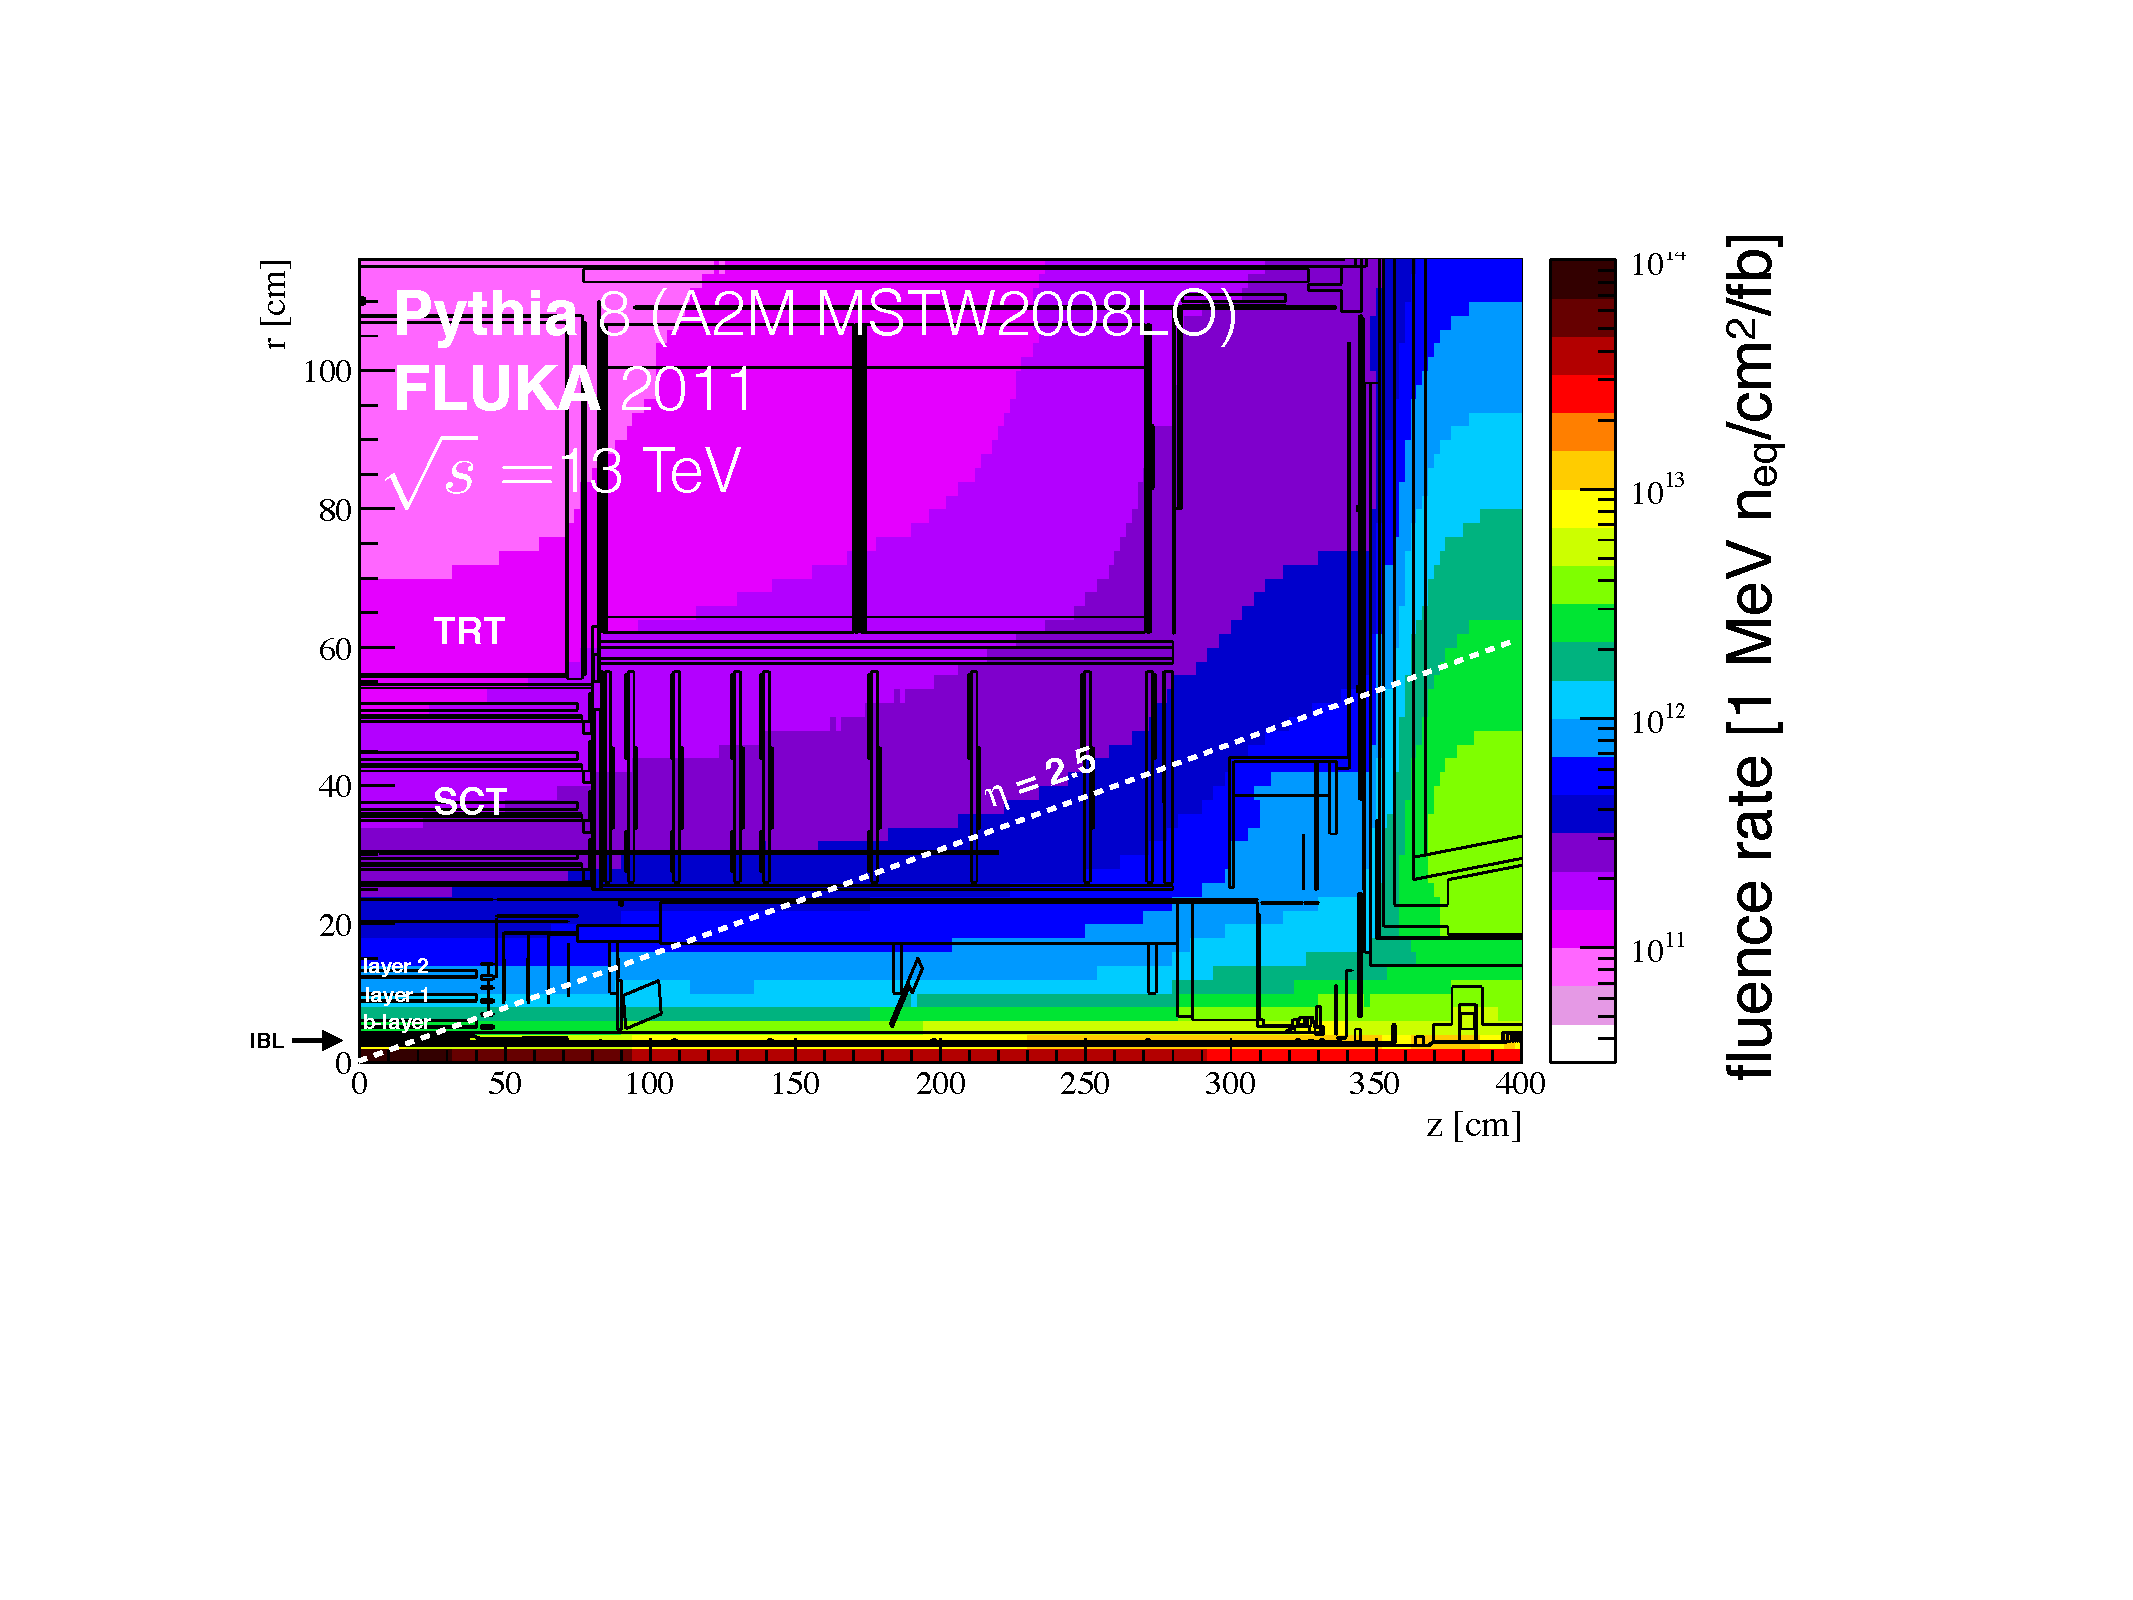
\includegraphics[width=0.6\textwidth]{Labeled2.pdf}
\caption{Simulated 1 MeV $n_\text{eq}$ fluence predictions shown as a function of the radial and longitudinal distance from the geometric center of the detector for a one-quarter slice through the ATLAS FLUKA geometry. Modeled are the pixel, SCT and TRT detector systems and services, and beyond $z = 350$ cm the end-cap calorimeter can be identified.}
\label{fig:fluenceoverview2}
\end{figure}

\begin{figure}[htpb!]
\centering
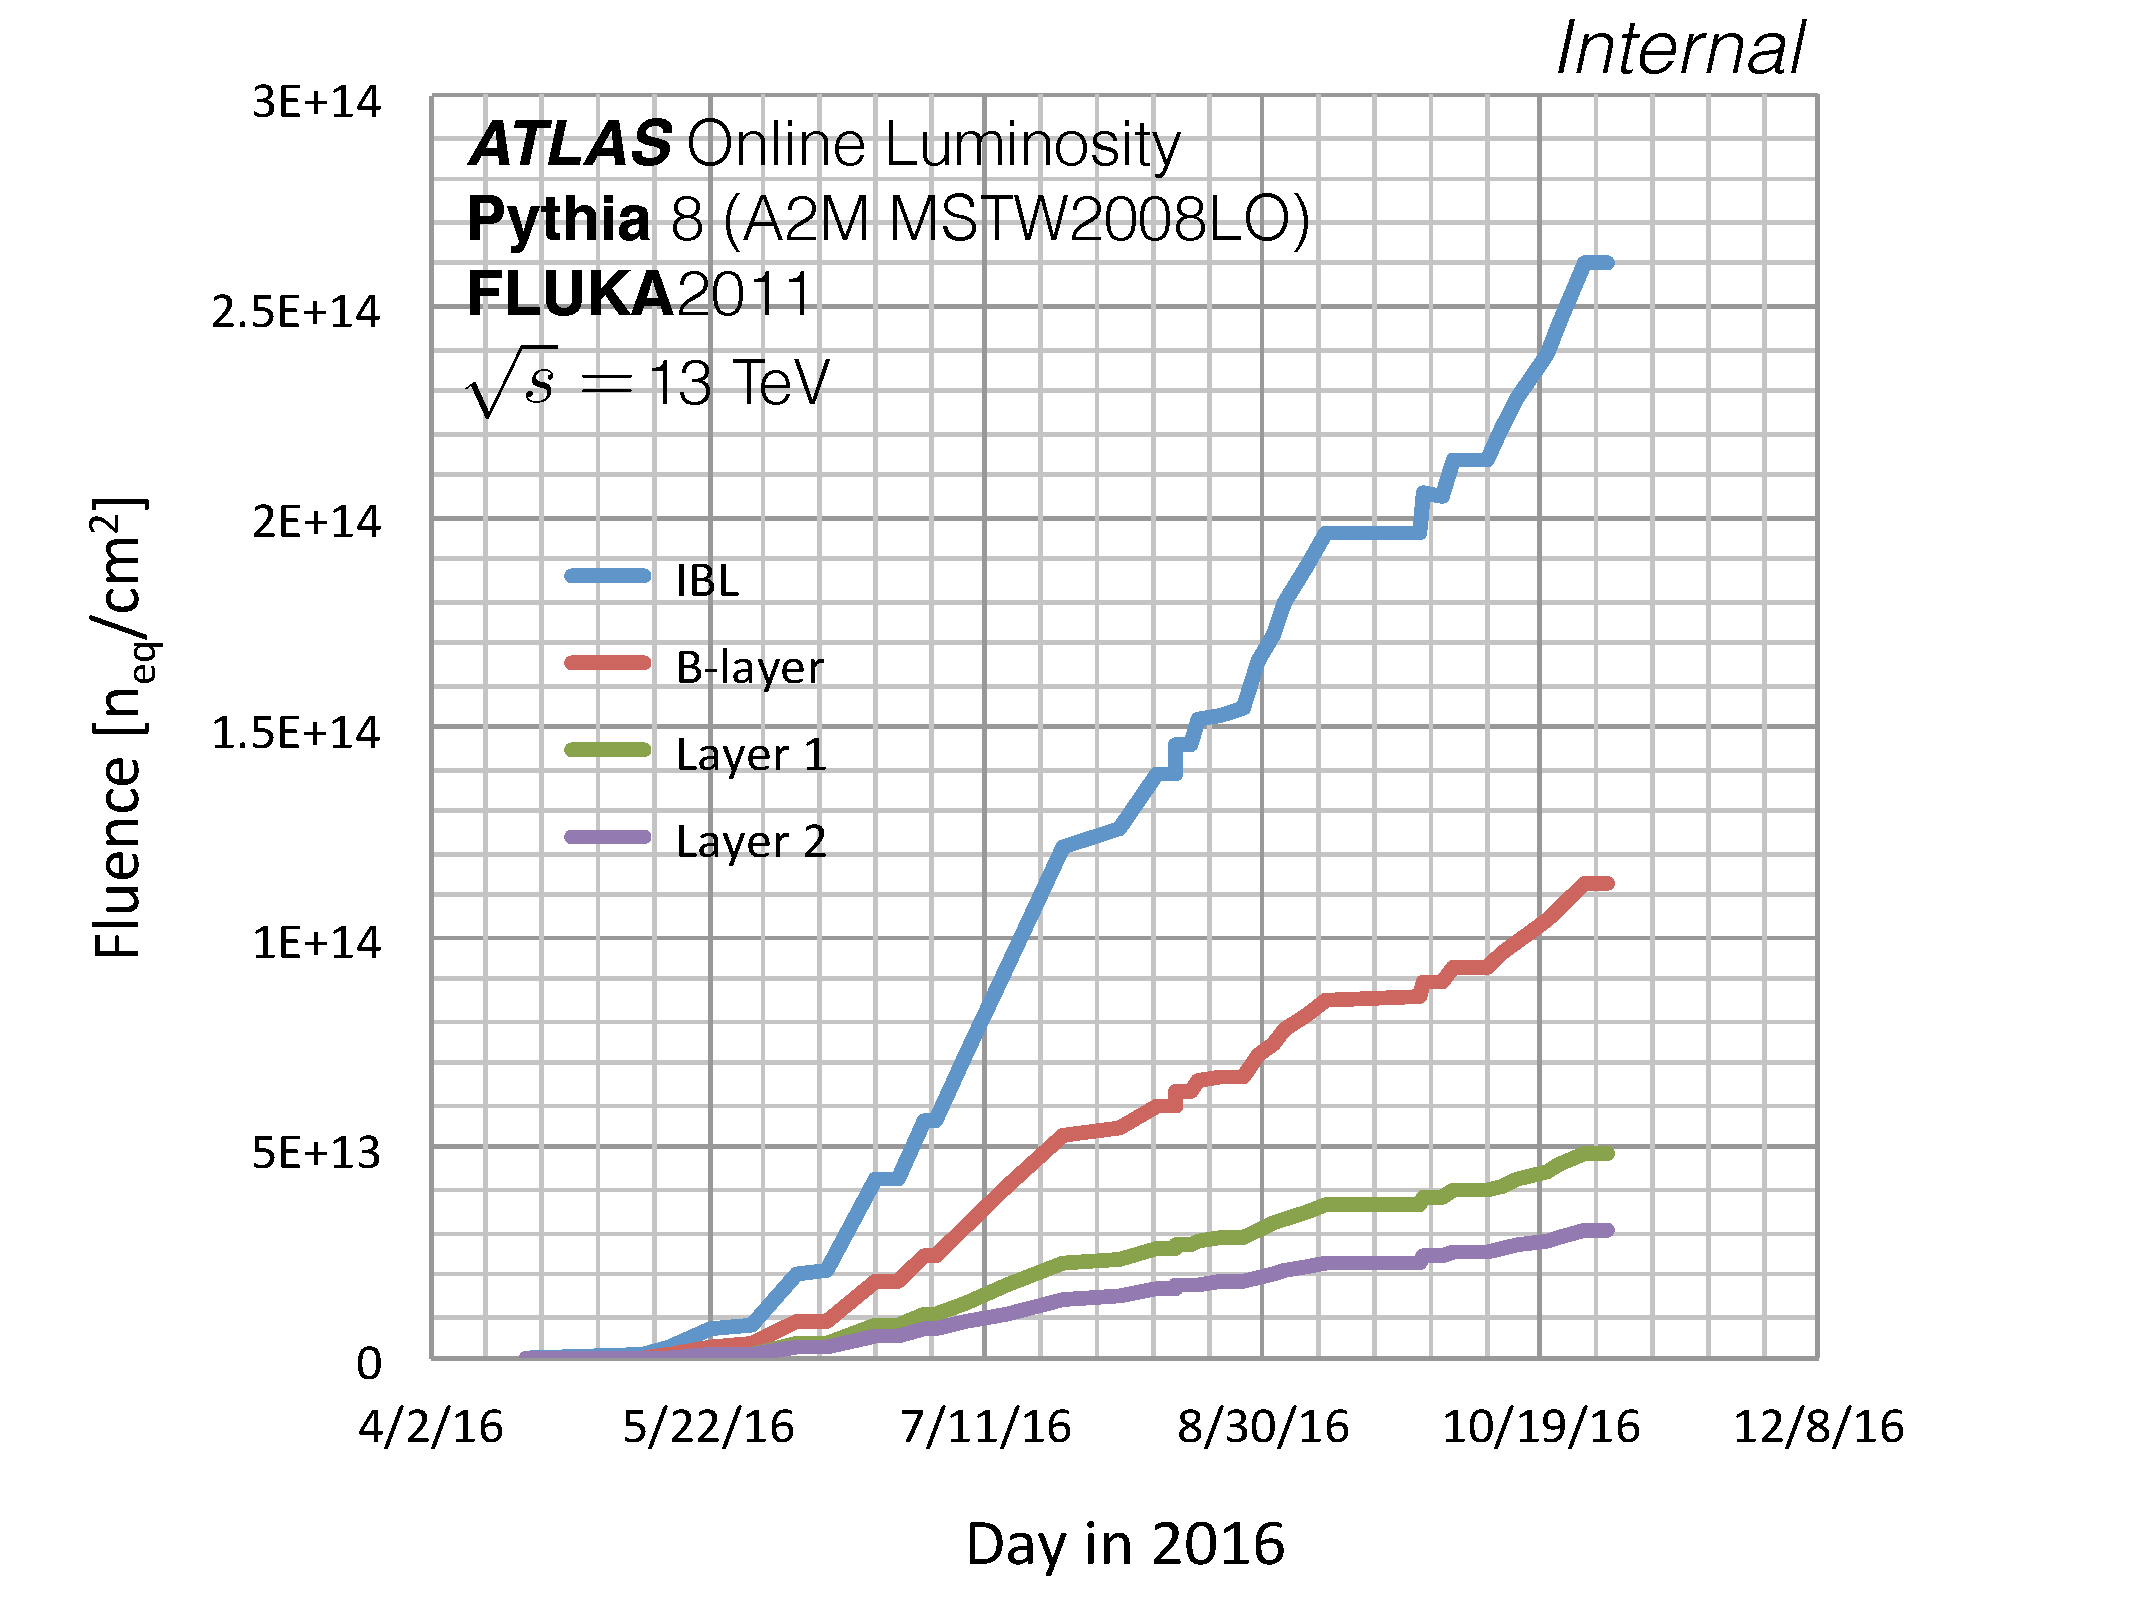
\includegraphics[width=0.49\textwidth]{Fluence_2016}
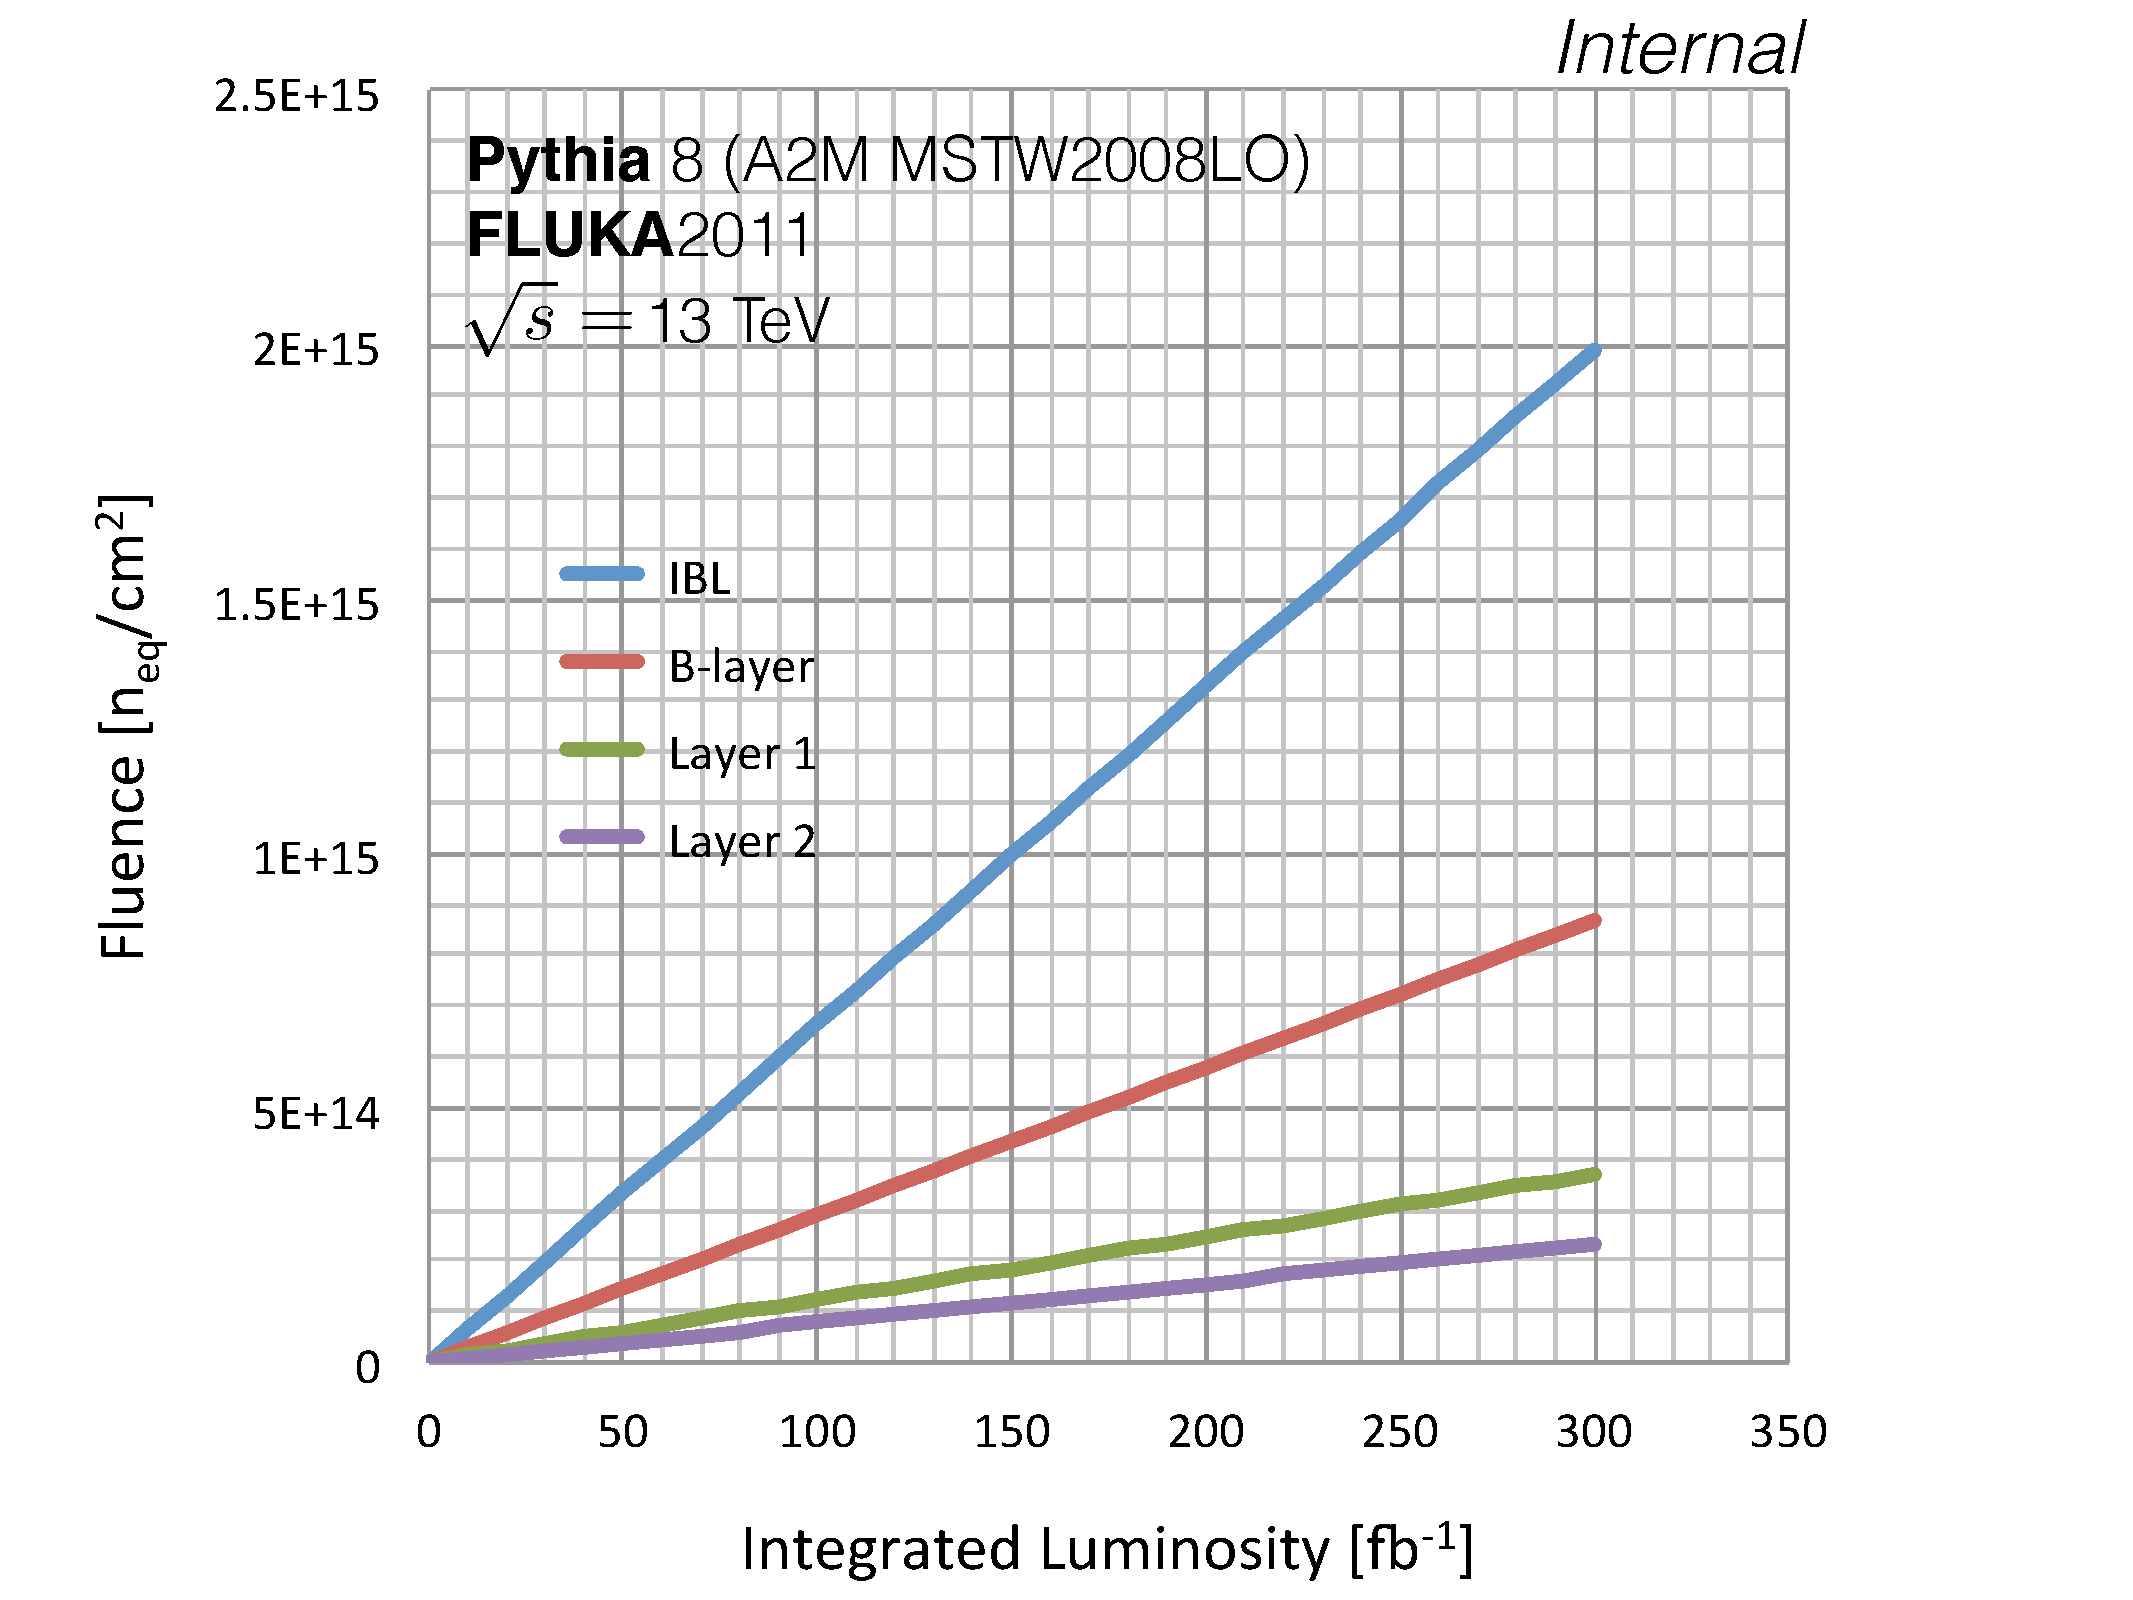
\includegraphics[width=0.46\textwidth]{Fluence_Run23.pdf}
\caption{Predictions for the fluence experienced by the four layers of the current ATLAS Pixel detector during Runs 2 and 3 of the LHC at $|\eta|\approx 0$.  The left plot shows the fluence accumulated during the 2016 run as a function of time while the right plot shows the fluences expected over all of Runs 2 and 3 as a function of integrated luminosity.}
\label{fig:fluenceoverview}
\end{figure}
  



The CMS collaboration has developed a model of radiation damage~\cite{Contardo:2020886,Swartz2002,Chiochia:2004qh,Swartz:2005vp}, validated with testbeam data, but is used to apply corrections to simulation from a model without inherent radiation damage effects.  The next section describes the physics of the digitization model and the first collision data comparisons are shown in Section~\ref{sec:digivalidation}.


\section{Full Digitizer Model}
\label{sec:fullmodel}

Figure~\ref{fig:app:raddamge1} presents a schematic overview of the physics models included in the digitization model.   
\begin{figure}[htpb!]
\centering
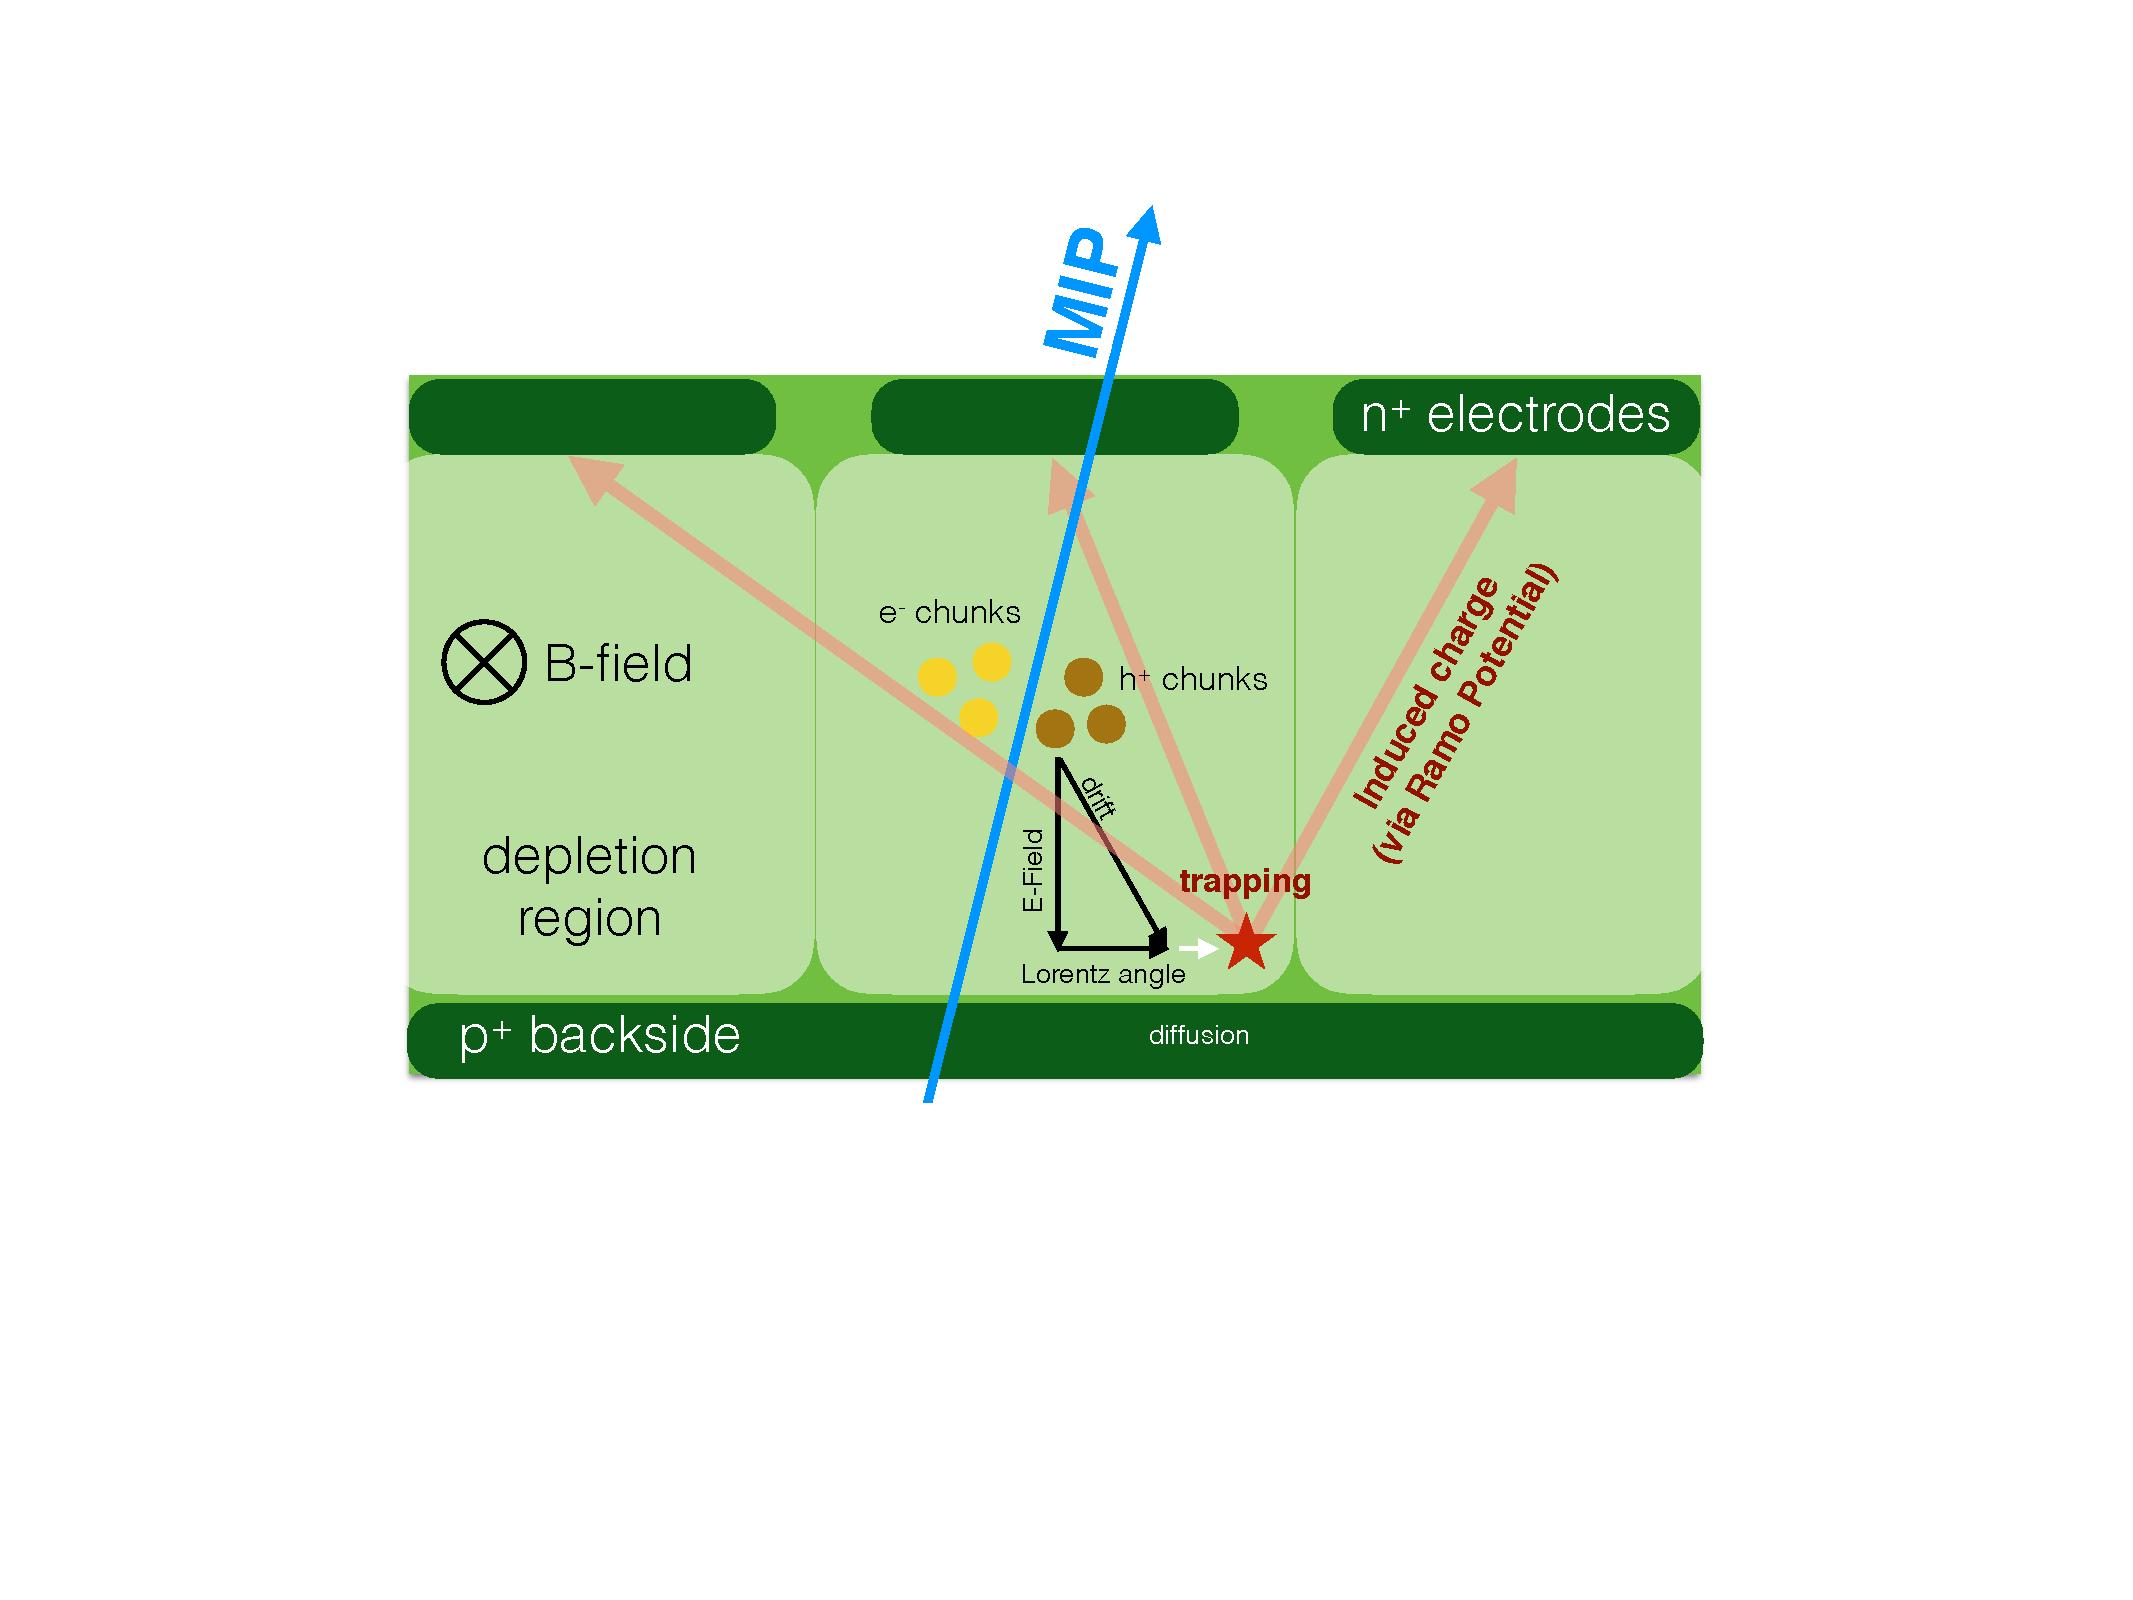
\includegraphics[width=0.95\textwidth]{DigitizerSchematic}
\caption{A schematic diagram illustrating the components of the digitizer model described in this note.  The blue line represents a minimum ionizing particle traversing the pixel sensor.  Chunks of electrons and holes, each representing $\mathcal{O}(10)$ fundamental charges, are transported to the electrodes.  Holes drift toward the backplane under the influence of the electric field and also experience transverse motion due to the magnetic field (deflecting at the Lorentz angle).  Thermal diffusion also changes the position of the charges.  Before being collected, electrons or holes may be trapped by defects in the silicon.  Even though the charge chunk may be trapped, it still induces a charge on the primary and neighbor electrodes via the Ramo potential.  }
\label{fig:app:raddamge1}
\end{figure}
Inputs to the digitizer are the detector geometry and conditions, including the 
fluence.  Input to the digitizer is an energy deposition from a charged particle 
too, produced by Geant4~\cite{Agostinelli:2002hh} (possibly with corrections for straggling in thin 
silicon~\cite{Bichsel:1988if}).  Technology Computer Aided Design (TCAD) is used to model the electric 
field, including radiation damage effects (Section~\ref{sec:ElectricField:SimulationDetails}).  An 
appropriate bias voltage is determined to ensure a large depletion region.  Ionization energy is converted into electron-hole pairs ($\sim 3.6$ 
eV/pair) which experience random motion from diffusion.  Chunks of fundamental charge carriers drift 
toward the electrode (electrons) or backplane (holes) under the influence of the electric field, with a 
field- and temperature-dependent mobility.  The number of fundamental charges per chunk is tuned to 
save time and a correction is applied to account for an over-estimation of fluctuations.  In addition to drifting toward the electrodes under the influence of the electric 
field, there is a transverse component to the drift due to the 2 T magnetic field in the ATLAS ID.  A field- 
and temperature-dependent Lorentz angle is combined with the mobility to compute the time for a 
charge carrier to be collected.  This time is compared to a 
fluence-dependent trapping time, the characteristic time a charge 
carrier will travel for before it is trapped.  If the drift time is longer than the trapping time, the chunk is 
declared trapped.  The location of the chunk at the trapped position is calculated based on the starting 
position and trapping time.  Since moving charges induce a current in the 
collecting electrode, signal is induced on electrodes from trapped charges as well.  This induced charge 
also applies to neighboring pixels, which contributes to charge sharing.  The induced charge from 
trapped chunks is calculated from the initial and trapped positions using a weighting potential.  The sum of the collected and induced charge is then converted into a ToT that is 
used by cluster and track reconstruction tools.

In what follows the luminosity to fluence conversion, the electric field modelization, the trapping effect 
and the weighting field implementation in the new digitization model are discussed.


\subsection{Luminosity to Fluence Conversion}
 The most important input to the radiation damage digitizer is the estimated NIEL.  
 Section~\ref{sec:expflu} introduced the baseline FLUKA simulation that is used to determine the 
 conversion factor between integrated luminosity and fluence. This prediction yields a conversion of
  about $59.6\times 10^{11}$ $n_\text{eq}/\text{cm}^2/\text{fb}^{-1}$ for the IBL and $29.2\times 10^{11}$ $n_\text{eq}/\text{cm}^2/\text{fb}^{-1}$ for the $b$-layer. In order to establish systematic uncertainties on these predictions, the fluence is converted into a prediction for the leakage current. The leakage 
current can be precisely measured and therefore provides a powerful constraint on the FLUKA simulation. For a time $t$ at constant temperature $T$ after an instantaneous irradiation with fluence $\Phi$, the predicted leakage current is given by Equation~\ref{eq:alpha_annealing} already presented 
in~Section\ref{sec:RadDam}.

The full leakage current is then estimated by discretizing time into four hour periods, averaging luminosity and temperature information if finer in a particular period, and then sum over time in Eq.~\ref{eq:alpha_annealing}.  This leads to a complication in the $\alpha_0$ parameter that has no explicit time dependence, but does depend on temperature.  One proposal\footnote{Another proposal is to sum the inverse temperatures~\cite{Barney:1709387}.  Such a method has been compared with Eq.~\ref{eq:leakage2} and results in similar predictions for the leakage current with the current fluence levels and annealing times.}~\cite{moll-thesis} is to absorb the temperature dependence in Eq.~\ref{eq:alpha_annealing} into the logarithm term as an effective scaling of the time axis:

\begin{align}
\label{eq:leakage2}
I_\text{leak}=V\cdot\Phi\cdot\left(\alpha_Ie^{-t/\tau}+\alpha_0^*-\beta\log(\Theta(T)t/t_0)\right),
\end{align}

\noindent where $\alpha_0^*=7.07\cdot 10^{-17}\;$A/cm is the value of $\alpha_0$ from Eq.~\ref{eq:alpha_annealing} evaluated at a reference temperature $T_\text{ref}=21^{\circ}$C and the time scaling function $\Theta(T)$ is defined by

\begin{align}
\label{eq:tempscaling}
\Theta(T) = \exp \left[ - \frac{E_I^*}{k_\text{B} } \left( \frac{1}{T} - \frac{1}{T_\text{ref} } \right) \right],
\end{align}

where $E_I^*=(1.3\pm 0.14)$ eV.  For a fixed time period with constant temperature, Eq.~\ref{eq:alpha_annealing} and Eq.~\ref{eq:leakage2} are mathematically identical.  However, the latter allows for a natural extension to non-constant temperature:

\begin{align}
\label{eq:leakage_modified}
I_\text{leak}=V\cdot\sum_{i=1}^n\cdot\phi_i\cdot t_i\cdot\left[\alpha_I\exp\left(-\sum_{j=i}^n\frac{t_j}{\tau(T_j)}\right)+\alpha_0^*-\beta\log\left(\sum_{j=i}^n\frac{\Theta(T_j)\cdot t_j }{ t_0}\right)\right],
\end{align}

where $\phi_i$ is the fluence rate, $t_i$ is the time in period $i$, and $T_i$ is the temperature in period $i$.  The first sum is over all time periods and the two sums inside the exponential and logarithm functions are over the time between the irradiation in time period $i$ and the present time.

Using the measured module temperature as a function of time, Eq.~\ref{eq:leakage_modified} is used to predict the leakage current as shown in Fig.~\ref{fig:leackagecurrent:beta}. Module properties were updated every ten minutes.  Since the IBL was newly inserted before the 2015 run, it is expected that the leakage current starts off at zero.  A constant luminosity-to-fluence conversion factor is fit to the data per module group in the dashed region near the end of the run.  Module groups differ by their distance along the beam direction from the geometric center of the detector.  The fitted prediction provides an excellent description of the data over the entire Run for all four module groups considered in Fig.~\ref{fig:leackagecurrent:beta}.  There is a clear $z$-dependence on the observed spectrum which is compared with the FLUKA predictions described in Sec.~\ref{sec:expflu} in Fig.~\ref{fig:leackagecurrent:eta}.  The predictions match the measured values well at $z=0$ with some deviations observed at higher $z$.  The remainder of this Section focuses on central $z$, using the FLUKA simulations without modification for the central value, but with a $15\%$ uncertainty on the fluence.  The ATLAS tracking acceptance is $|\eta|<2.5$, which corresponds to $z\approx 20$ cm in the IBL.

\begin{figure}[h!]
\centering
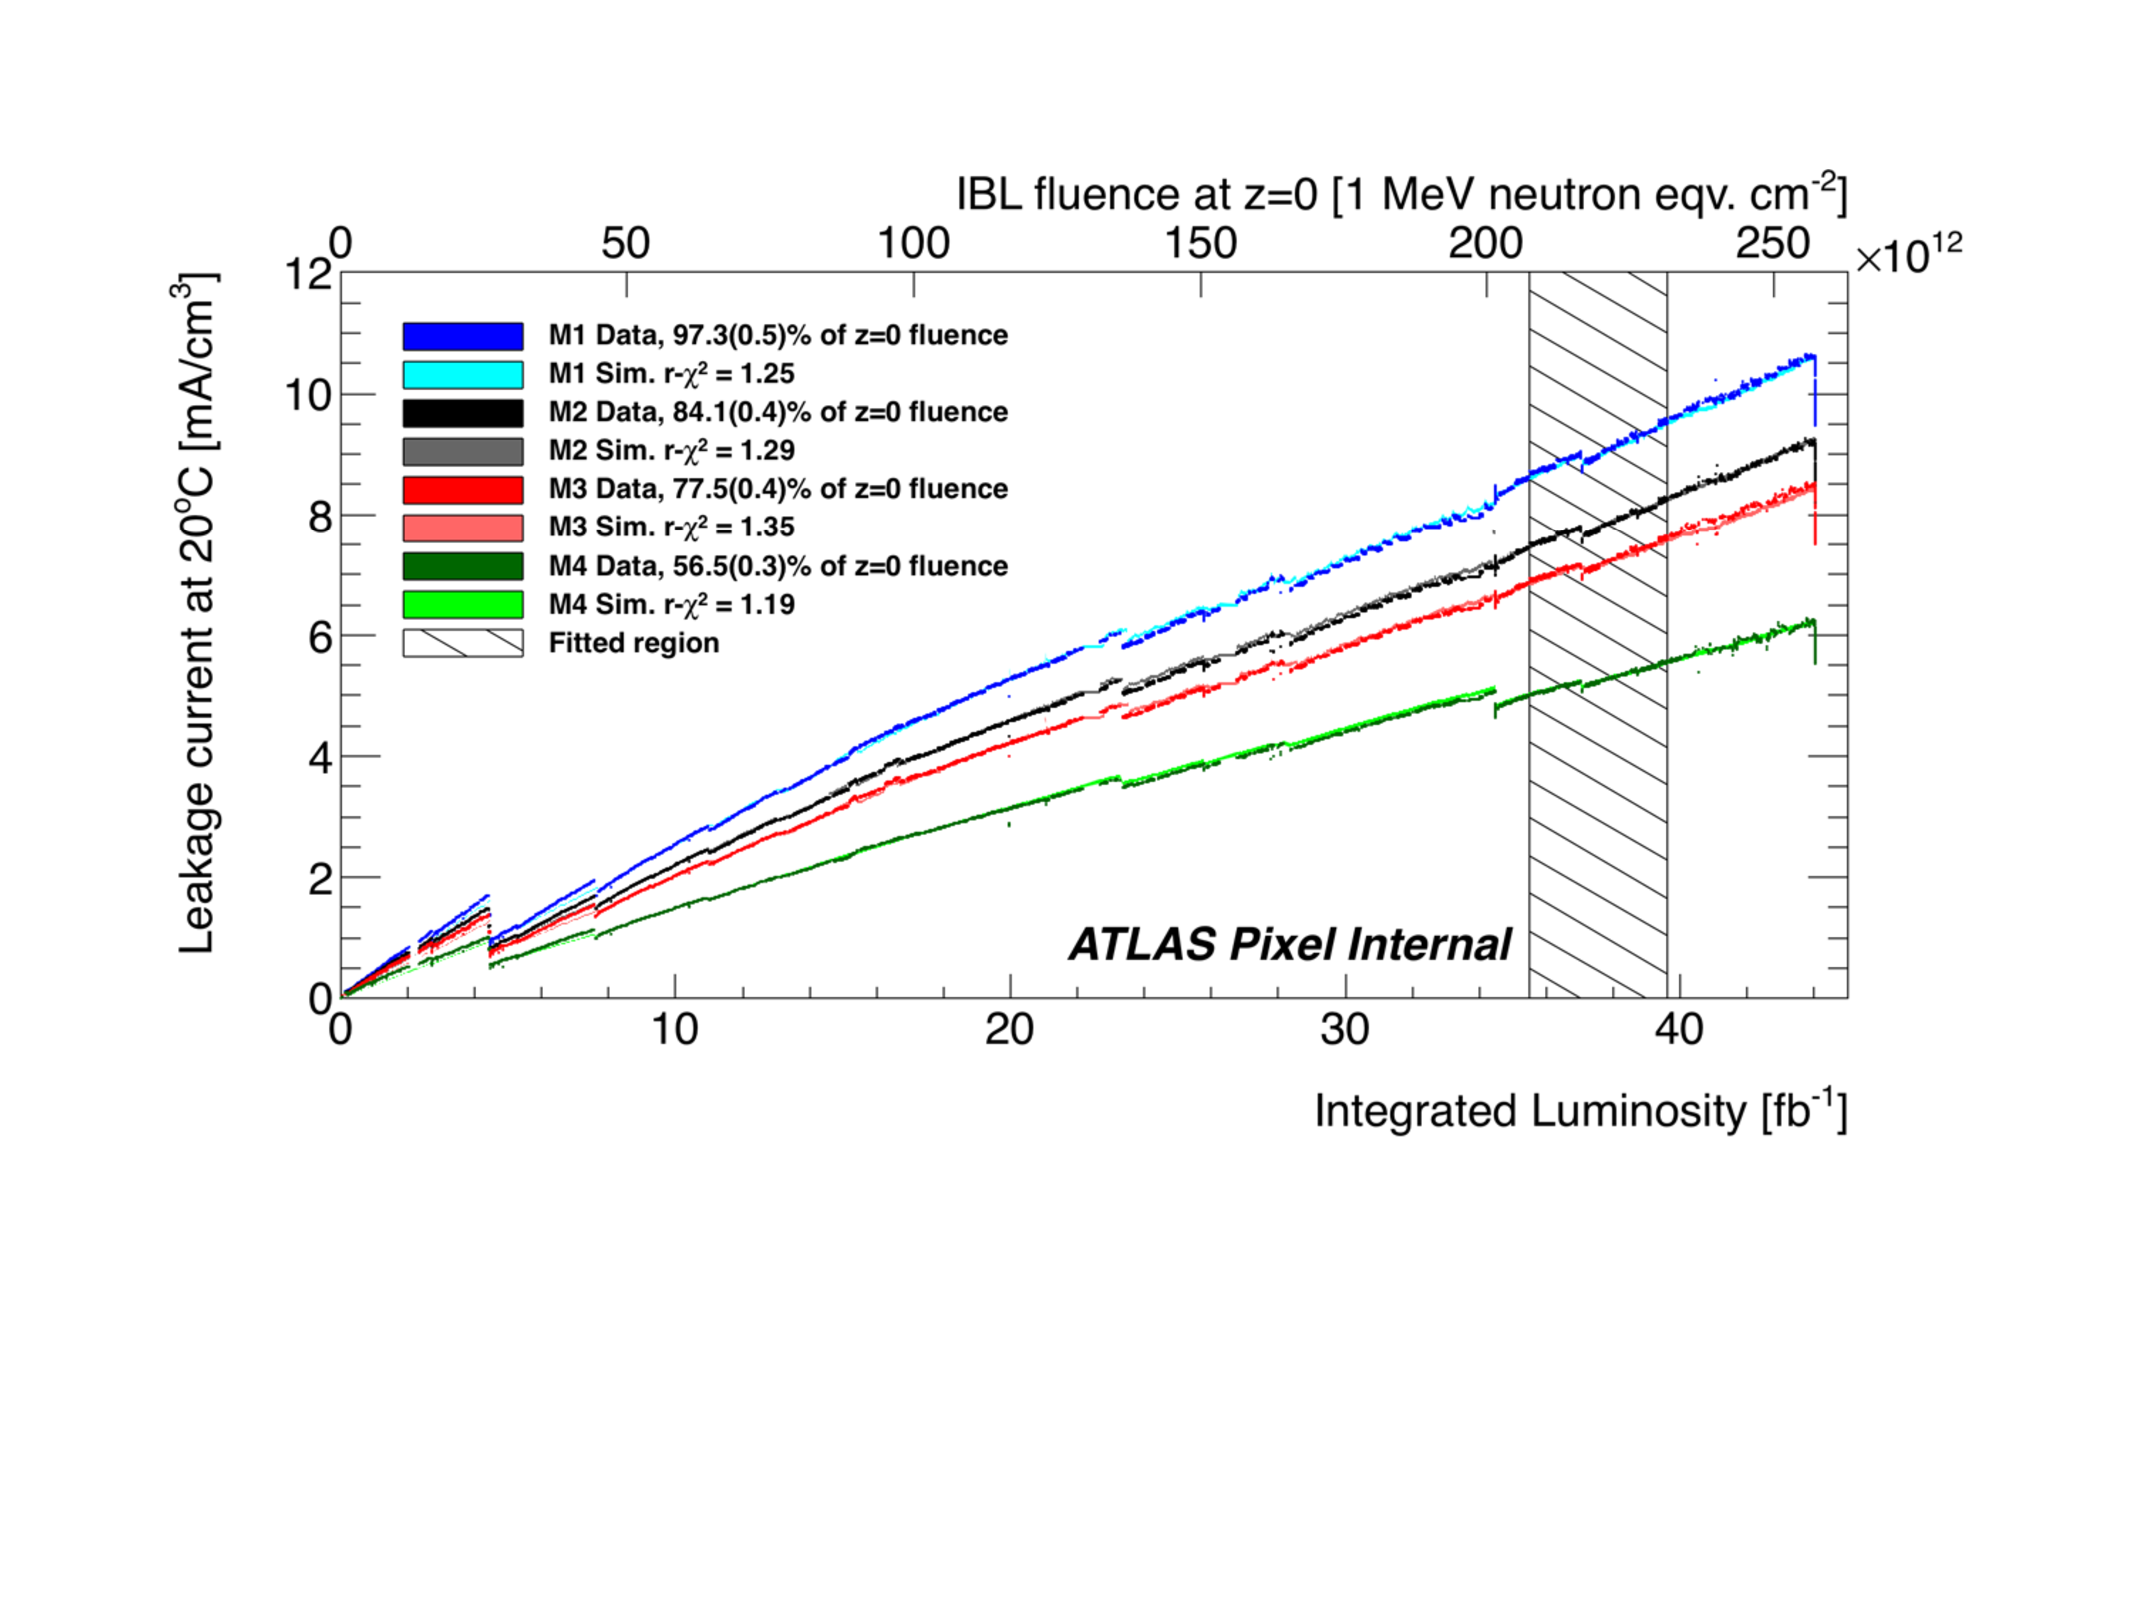
\includegraphics[width=0.85\textwidth]{leakagecurrent_Dann.pdf}
\caption{The measured and predicted leakage current for the IBL as a function of date since the start of the 2015 data run, based on Eq.~\ref{eq:leakage_modified}.   Current spikes and the first and last 200 luminosity blocks of each run are excluded. The leakage current is normalized to a temperature of $20^{\circ}$C. The dashed region indicates the normalization region for the fit for the luminosity-to-fluence conversion factor per module group. Each module group is $8$ cm long on each side of the detector along the beam direction.  The groups M1, M2, M3 approximately span the ranges $z\in[-8,8]$ cm, $|z|\in[8,16]$ cm, and $|z|\in [16,24]$ cm, respectively. }
\label{fig:leackagecurrent:beta}
\end{figure}

\begin{figure}[h!]
\centering
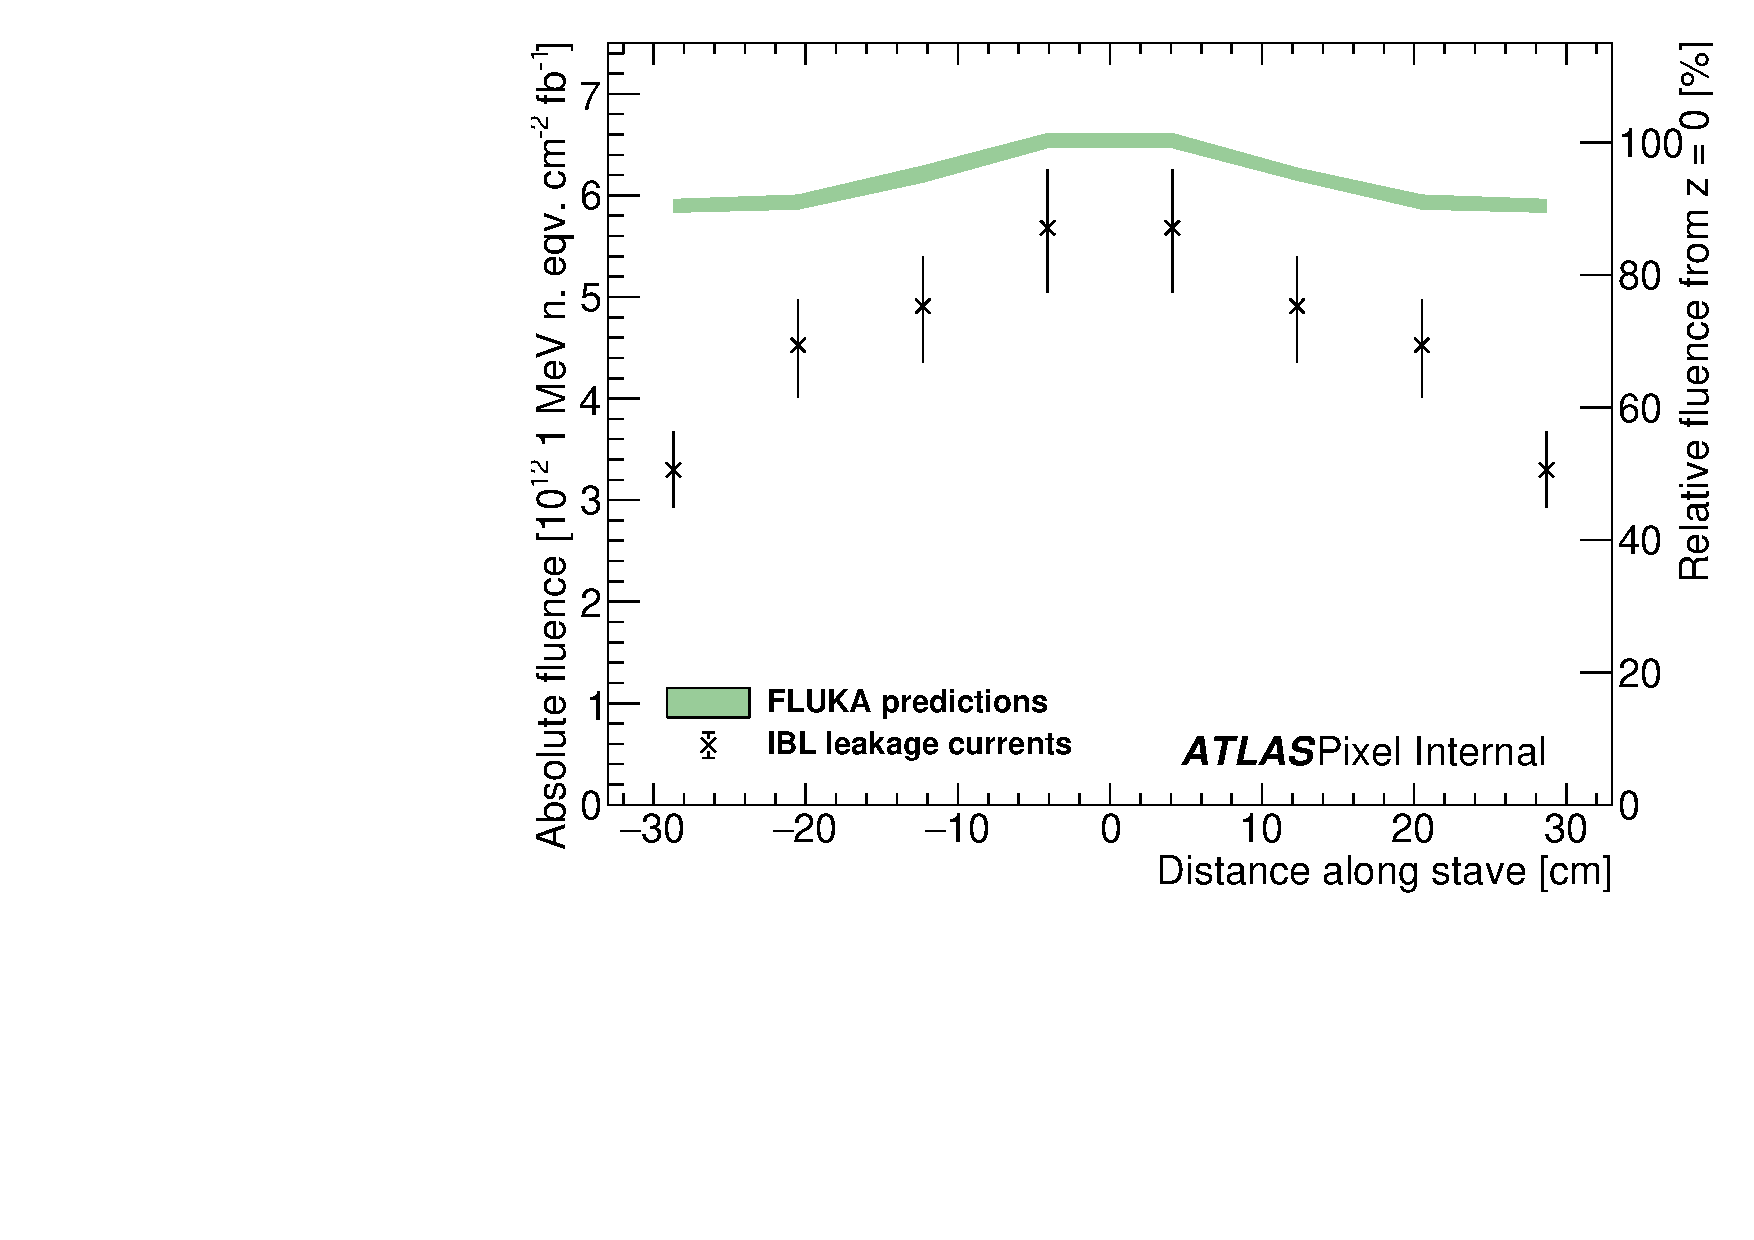
\includegraphics[width=0.65\textwidth]{simulation-FLUKA-absolute.pdf}
\caption{The fluence-per-luminosity conversion factors extracted from leakage current fits as a function of z, compared with the FLUKA predictions described in Sec.~\ref{sec:expflu}. The leakage current error bars are dominated by a conservative $10\%$ uncertainty, accounting for the variation in the bias voltage at full depletion~\cite{ATL-INDET-PUB-2014-006}.  Uncertainties due to the annealing model ($0.1\%$) and data fit ($0.5\%$) are subdominant.}
\label{fig:leackagecurrent:eta}
\end{figure}

\subsection{Electric Field Modelization}
The radiation-induced states in the silicon band gap affect the electric field in the pixel cells by altering 
the electric field distribution in the bulk\footnote{There are also changes at the surface, but the focus 
here is on the deformations on the electric field within the sensor.}. Since many variables used in signal 
formation calculations depend on the electric field (drifting time, Lorentz angle deviation, etc.), including 
radiation damage effects requires a careful parameterisation of the electric field in the pixels. 
Investigation of the electric field profile in the bulk of irradiated silicon sensors have shown that for 
certain materials, the electric field is no longer linear with the bulk depth after irradiation.  
In what follows a default model used for subsequent 
studies will be introduced but references to alternative models in the literature are discussed.   The fluence-dependent 
depletion voltage calculation is presented in Sec.~\ref{sec:depletionvoltage} and the resulting field 
profiles are shown in Sec.~\ref{sec:Efieldprofile}.  Section~\ref{sec:Efieldmodelcomparisons} provides a 
brief comparison between the default model and alternative models.

\section{Full Digitizer Predictions and Validation}
\label{sec:digivalidation}

\section{Full Digitizer: Summary and Perspectives}
\label{sec:digiconclusions}
